\documentclass[11pt]{article}
\usepackage{classTools}

\drafttrue

\begin{document}

% To include a problems set header, use the psHeader command
\psHeader{4}{Wed Oct. 12, 2022 (11:59pm)}

\textbf{Your name: Andrew Courtney}

\textbf{Collaborators: }

\textbf{No. of late days used on previous psets: 5}

\textbf{No. of late days used after including this pset: 5}

\begin{enumerate}
    \item (Randomized Algorithms in Practice)  
    \begin{enumerate}
        \item Implement Randomized QuickSelect, filling in the template we have given you in the \href{https://github.com/Harvard-CS-120/cs120/tree/main/fall2022/psets}{Github repository}.  
        
        \item 
        In the repository, we have given you datasets $x_n$ of key-value pairs of varying sizes to experiment with.  For each dataset $x_n$ and any given number $k$, you will compare two ways of answering the $k$ selection queries
        Select$(x_n,[n/k])$, Select$(x_n,[2n/k]), \ldots$, Select$(x_n,[(k-1)n/k])$ on $x_n$, where $[\cdot]$ denotes rounding to the nearest integer:
        \begin{enumerate}
            \item Running Randomized QuickSelect $k$ times
            \item Running MergeSort (provided in the repository) once and using the sorted array to answer the $k$ queries
        \end{enumerate}
        Specifically, you will compare the {\em distribution} of runtimes of the two approaches for a given pair $(n,k)$ by running each approach many times and creating density plots of the runtimes.  The runtimes will vary because Randomized QuickSelect  is randomized, and because of variance in the execution environment (e.g. what other processes are running on your computer during each execution).
        
        We have provided you with the code for plotting. Before plotting, you will need to implement MergeSortSelect, which extends MergeSort to answer $k$ queries. Your goal is to use these experiments and the resulting density plots to propose a value for $k$, denoted $k^*_n$, at which you should switch over from Randomized QuickSelect to MergeSort for each given value of $n$. Do this by experimenting with the parameters for $k$ (code is included to generate the appropriate queries once the $k$s are provided) and generate a plot for each experiment.  Explain the rationale behind your choices, and submit a few density plots for each value of $n$ to support your reasoning.  (There is not one right answer, and it may depend on your particular implementation of QuickSelect.) 
        
        
\begin{proof}
We go to the attached chart. \\
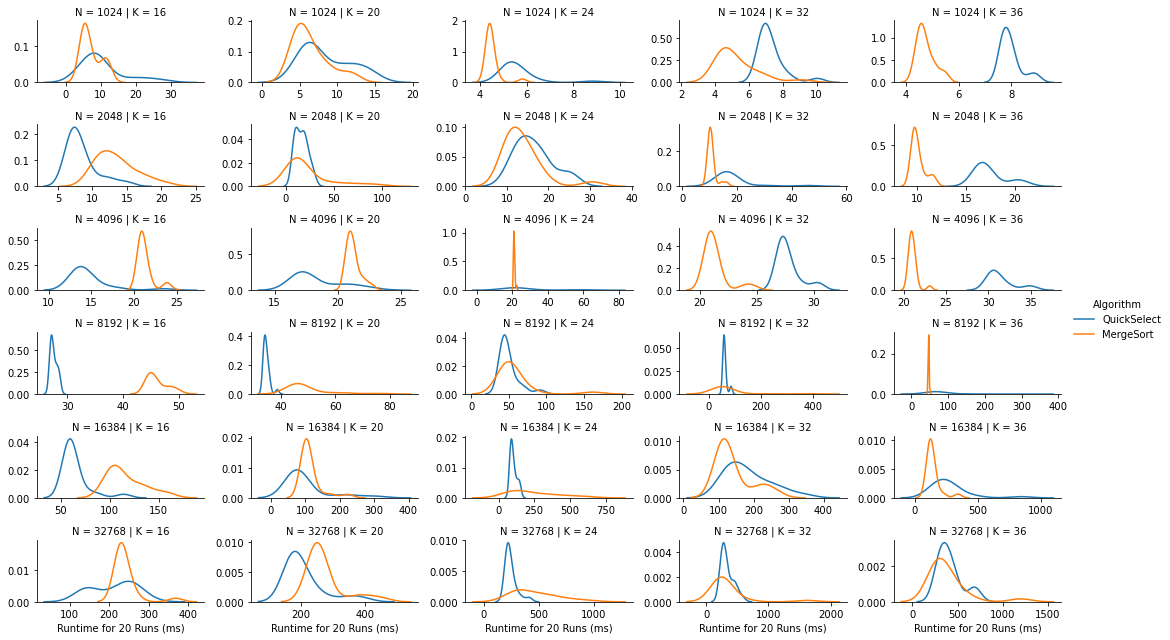
\includegraphics[width=6in]{1-14}

It's a little squeezed together, but I think we get the point. Generally, the larger $K$ gets, the better MergeSort becomes. It's tougher to tell with $N$ increasing, but generally QuickSelect becomes more appealing when that happens from the graphical data (this makes sense asymptotically, because $O(n \log n)$ is punished more than $O(n)$ by $n$ increasing). So we can look at specific cases now.

For $N = 1024$, $k^*_{1024} = 16$, because $K = 20$ already features MergeSort outperforming QuickSelect. For $N = 2048$, $k^*_{2048} = 20$ looks good. For $N = 4096$, $k^*_{4096} = 24$ has a weird plot but is the only one that really lines up. For $N = 8192$, I'd pick something in the range of $k^*_{8192} = 26$ and split the difference. For $N = 16384, k^*_{16384} = 30$ seems like a good choice, and then we can end with $k^*_{32768} = 32$. So in general these values of $k^*_n$ are increasing pretty evenly with the values of $K$ that we've chosen.
\end{proof}

        \item Extrapolate to come up with a simple functional form for $k^*_n$, e.g. something like $k^*(n)=3\sqrt{n}+6$ or $k^*(n)=10\log n$. (Again there is not one right answer.)
        
        
\begin{proof}
It looks like the best answer here will involve a logarithm just because our values increase pretty evenly with powers of two. Given that $\log_2 1024 = 10$ and $\log_2 32768 = 15$, we can get pretty close and chalk up the differences to small sample size error if we use the form
$$
k^* (n) = 3 \ln (n),
$$

given that this returns $k^*_{1024} = 21, k^*_{32768} = 32$, and distributes the rest of the results fairly evenly. I prefer

$$
k^* (n) = 2 \log_2 (n)
$$

as a model, because $2$ is a much nicer number in computer science. This gives us $k^*_{1024} = 20, k^*_{32768} = 30$, and regulates the middle fairly well.
\end{proof}

        \item (*optional)  One way to improve Randomized QuickSelect is to choose a pivot more carefully than by picking a uniformly random element from the array. A possible approach is to use the \textit{\textbf{median-of-3}} method: choose the pivot as the median of a set of 3 elements randomly selected from the array. Add Median-of-3 QuickSelect to the experimental comparisons you performed above and interpret the results.
        

\begin{proof}
See below. \\
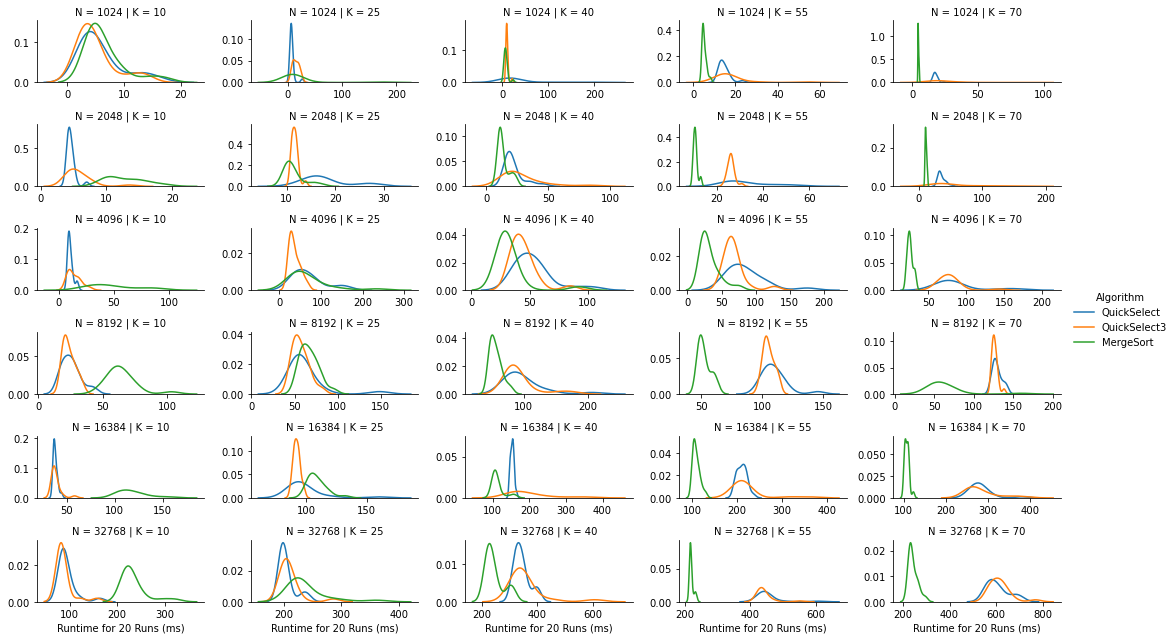
\includegraphics[width=6in]{1-13}
\end{proof}

As we can see here, Median-of-3 QuickSelect does comparatively worst when $K$ is small (because it requires us to do more operations) and when $N$ gets large (because it's harder to generate a random number). However, in most cases it blows the other algorithms out of the water because the sorting process becomes much faster, and so it outperforms QuickSelect most as $K$ increases. 
    \end{enumerate}


    \item (Dictionaries and Hash Tables) 
    Recall the DuplicateSearch problem from Lecture 3. Show that DuplicateSearch can be solved by a Las Vegas algorithm with expected runtime $O(n)$ using a dictionary data structure.  (You can quote the runtimes of the implementation of a dictionary data structure from Lecture 9 without proof.) 
    
\begin{proof}
We use the implementation of the dictionary described in Lecture 9. Define a random hash function $h$ which takes inputs from the size of the universe of objects with a duplicate and returns a number in the range of $(0, m)$ for some $m$ we define. It takes $O(1)$ time to generate and store $h$, and each time we calculate $h(x)$ for some $x$ it takes time $O(1)$. To search our dictionary, it takes time $O(1 + n/m)$, which becomes the same as $O(1)$ as long as $m = \Omega (n)$, which we can easily define here (in fact, we did this without problem in class). So we have a Las Vegas algorithm that uses a dictionary data structure, as we are asked.

Here is our algorithm: first we generate and store $h$ in $O(1)$ time. Then for each $x$ in the input set of size $n$, we first search to see if $x$ has been hashed in time $O(1)$; if so, we return that element (because we know it to be a duplicate). If not, we hash it in time $O(1)$. We do this at most $n$ times, which means that we do a maximum of $2n - 1$ operations; therefore, the runtime for our algorithm overall is $O(n)$, as desired.
\end{proof}

\item  (Rotating Walks)       
    Suppose we are given $k$ digraphs on the same vertex set, $G_0=(V,E_0), G_1=(V,E_1), \ldots, G_{k-1}=(V,E_{k-1})$.  For vertices $s,t\in V$, a {\em rotating walk} with respect to $G_0,\ldots,G_{k-1}$ from $s$ to $t$ is a sequence of vertices $v_0,v_1,\ldots,v_{\ell}$ such that $v_0=s$, $v_\ell=t$, and $(v_i,v_{i+1})\in E_{i \bmod k}$ for $i=0,\ldots,\ell-1$.  That is, we are looking for walks that rotate between the digraphs $G_0,G_1,\ldots,G_{k-1}$ in the edges used.
    \begin{enumerate}
    
        \item Show that the problem of finding a Shortest Rotating Walk from $s$ to $t$ with respect to $G_0,\ldots,G_{k-1}$ 
        can be reduced to Single-Source Shortest Walks via a reduction that makes one oracle call on 
        a digraph $G'$ with $kn$ vertices and $m_0+m_1+\cdots+m_{k-1}$ edges, where $n=|V|$ and $m_i=|E_i|$.
        We encourage you to index the vertices of $G'$ by pairs $(v,j)$ where $v\in V$ and $j\in [k]$. 
        Analyze the running time of your reduction and deduce that the Shortest Rotating Walk can be found in time $O(kn+m_0+\cdots+m_{k-1})$.
       To test your reduction and algorithm, try running through the example in Part~\ref{part:BFS}.  \label{part:ReduceToOrdinary} 
       
\begin{proof}
We construct a digraph $G'$ with $kn$ vertices that are each labeled with an ordered pair $(v, j)$ where $v \in V$ and $j \in 0, 1, \dots, k - 1$ (the size is what I claim because $n = |V|$). Then we transfer edges from our graphs $G_0, \dots, G_{k - 1}$ to $G'$ by drawing an edge between $(v_m, j)$ and $(v_n, j + 1)$ if there exists an edge from $v_m$ to $v_n$ on the graph $G_j$ and $j < k - 1$; if $j = k -1$ and there exists an edge from $v_m$ to $v_n$ on $G_j$, then we draw an edge from $(v_m, j)$ to $(v_n, 0)$ on $G'$. 

This works as a transformation because this digraph only contains edges that describe moves that we can make in a Shortest Rotating Walk algorithm, and it contains every such move (as described by the process of creating the graph above). Now we test the runtime.

Knowing that we can use BFS to find the Single-Source Shortest Walk of a graph from class, we rely on the idea that if some graph $G$ has $n$ vertices and $m$ edges, we have a runtime of $O(n + m)$ when implementing the algorithm. We listed above that $G'$ has $kn$ vertices, so the first term is taken care of. For our second term, every single edge in each graph $G_i$ goes to $G'$ and there is no edge in $G'$ that is not in a graph $G_i$. Therefore the number of edges in $G'$ is the sum of the numbers of edges in each $G_i$, which means we get a runtime $G(kn + m_0 + \dots + m_{k - 1})$, as desired.
\end{proof}
        
        \item Run your algorithm from Part~\ref{part:ReduceToOrdinary} on the following pair of graphs $G_0$ and $G_1$ to find the Shortest Rotating Walk from $s=a$ to $t=c$; this will involve solving Single-Source Shortest Walks on a digraph $G'$ with $2\cdot 8=16$ vertices. Fill out the table provided below with the BFS frontier in $G'$ at each iteration, labelling the vertices of $G'$ as $(a, 0),(b, 0),\ldots,(g,0),(a,1),(b,1),\ldots,(g,1)$, and for each vertex $v$ in the table, drawing an arrow in the graph from $v$'s BFS predecessor to $v$.  \label{part:BFS}
%        \salil{is this the same example as from last year?  May be good to change it.} \salil{where's the table?}

            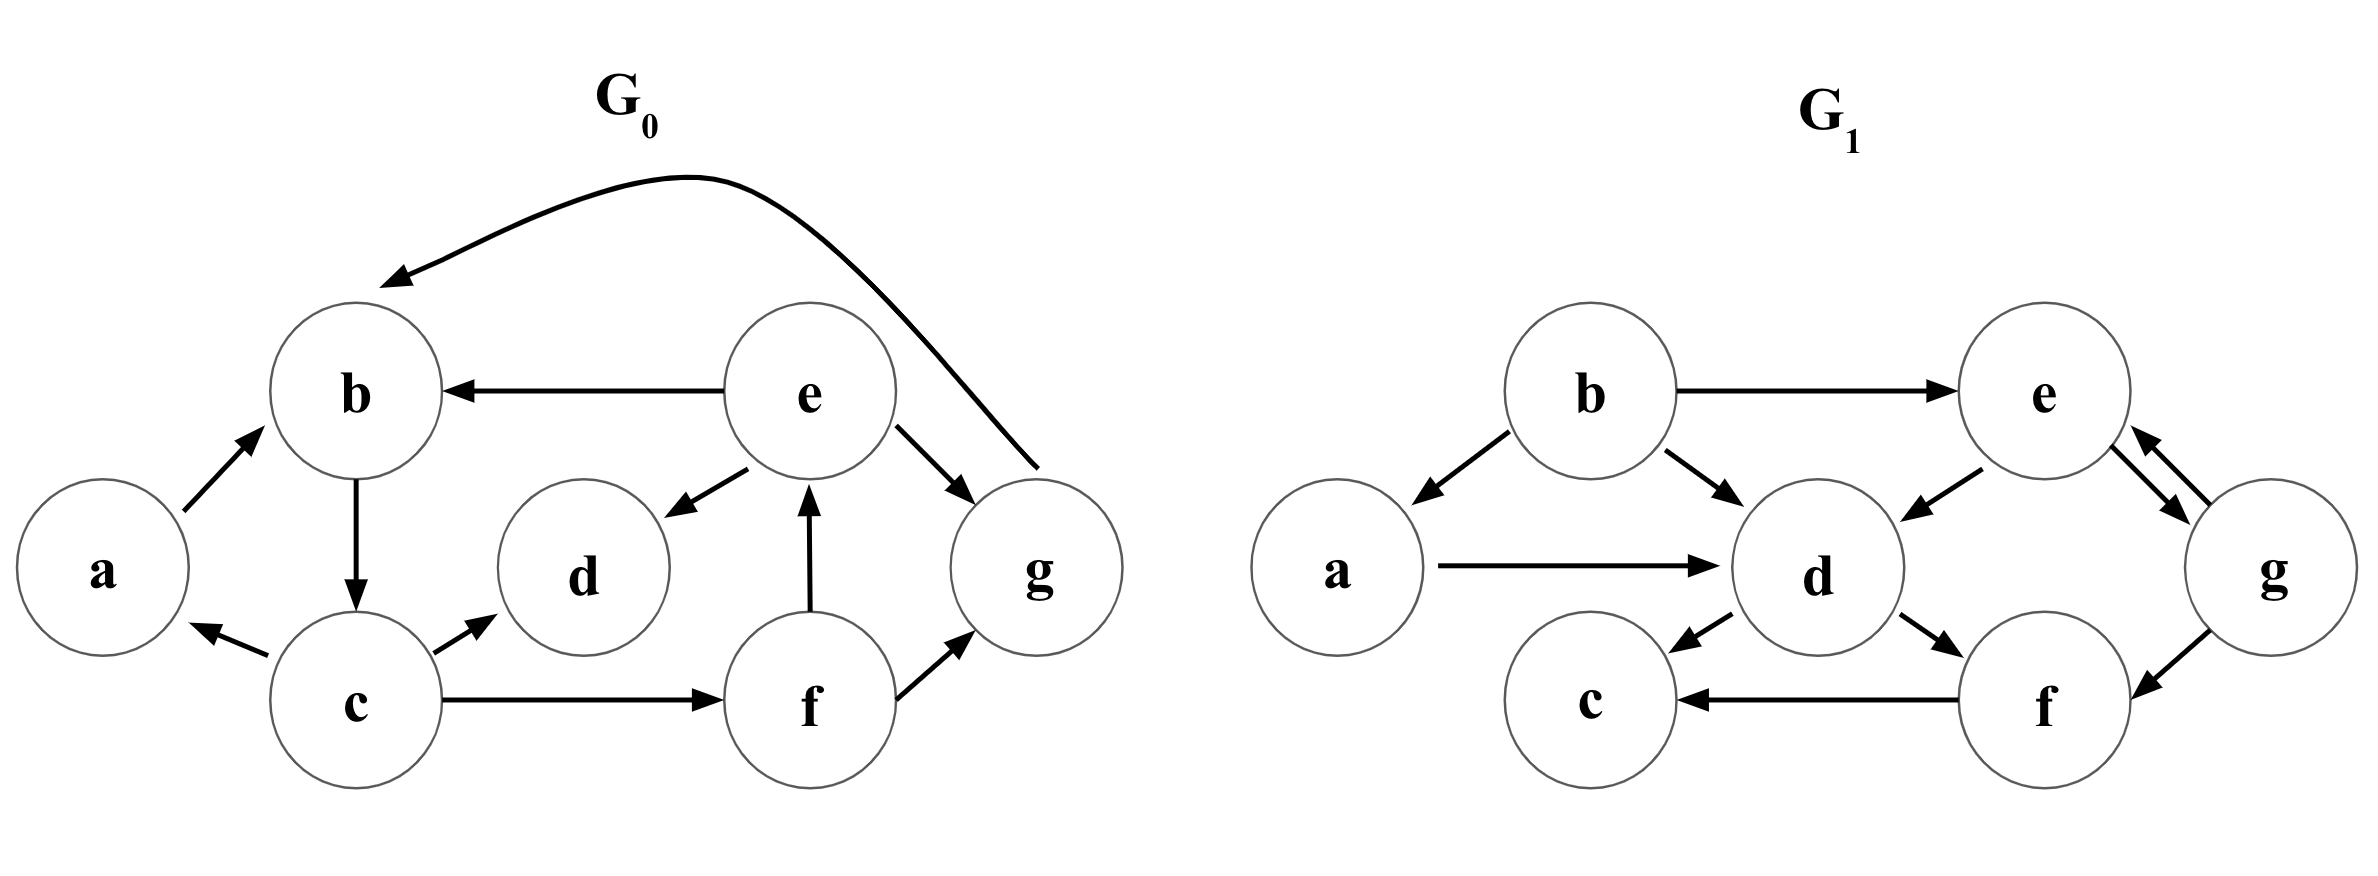
\includegraphics[width=14cm]{ps4_graphs_new.png}

\begin{proof}
        \begin{table}[ht]
        \centering
        \begin{tabular}{c|c|c}
            $d$ & Frontier $F_d$& Predecessor Relationships \\
            \hline
              0 & $(b, 1)$ & \\
              1 & $(d, 0), (e, 0)$ & $(a, 0) \to (b, 1)$ \\
              2 & $(d, 1), (g, 1)$ & $(b, 1) \to (d, 0), (b, 1) \to (e, 0)$ \\
              3& $(c, 0), (f, 0)$ & $(e, 0) \to (d, 1), (e, 0) \to (g, 1)$ \\
        \end{tabular}
    \end{table}
    
Therefore the Shortest Rotating Walk has length 4 here, with path $(a, 0) \to (b, 1) \to (e, 0) \to (d, 1) \to (c, 0)$, where we make a move four times.

\end{proof}

    \item 
        A group of three friends decides to play a new cooperative game (similar to the real-life board game Magic Maze).  They rotate turns moving a shared single piece on an $n\times n$ grid.  The piece starts in the lower-left corner, and their goal is to get the piece to the upper-right corner in as few turns as possible.  Many of the spaces on the grid have visible bombs, so they cannot move their piece to those spaces.  Each player is restricted in how they can move the piece.  Player 0 can move it like a chess-rook (any number of spaces vertically or horizontally, provided it does not cross any bomb spaces). Player 2 can move it like a chess bishop (any number of spaces diagonally in any direction, provided it does not cross any bomb spaces).  Player 3 can move it like a chess knight (move to any non-bomb space that is two steps away in a horizontal direction and one step away in a vertical direction or vice-versa).   Using Part~\ref{part:BFS}, show that given the $n\times n$ game board (i.e., the locations of all the bomb spaces), they can find the quickest solution in time $O(n^3)$.  
        (Hint: give a reduction, mapping the given grid to an appropriate instance $(G_0,G_1,\ldots,G_{k-1},s,t)$ of Shortest $k$-Rotating Paths.)
        
        
\begin{proof}

This game reduces to the Shortest Rotating Walk problem, which we know already reduces to the Single-Source Shortest Walk problem. Label the $n \times n$ with some ordering such that every square has unique value between $0$ and $n^2 - 1$. Then the set of moves that each player can make can be modeled as a digraph with $n^2$ nodes and edges between any two nodes which the player is allowed to move to. In practice, this means that an edge from $v_m$ to $v_n$ exists if the appropriate chess move in that direction exists (for $G_1$, this is a move along a row or column; for $G_2$, a move two spaces in one direction and one space perpendicularly; for $G_3$, a move along a diagonal) and that no bomb exists on $v_m$ or $v_n$. Then we have defined $G_0, G_1, G_2$. Lastly, let $s$ be the bottom-left square (which in our numbering can have index 0) and $t$ be the top-right square (which can have index $n^2 - 1$).

This is an entirely correct way to represent the problem. First note that every single edge in a given graph $G_i$ represents a move that's possible in the original problem by definition; too, every move that's possible gets represented in $G_i$ because it's impossible to move to or from a bomb. Finally, each player rotates a turn on the same board, so the rotating walk idea is preserved. So the road forward is pretty straightforward from 3a and 3b - we convert $G_0, G_1, G_2$ to $G'$ as described there and then find the shortest path in time $O(n' + m')$, where $n'$ is the number of nodes in $G'$ and $m'$ is the number of its edges.

So now we can find runtime. Each $G_i$ has $n^2$ nodes so $G'$ has $3n^2$ nodes. Then we count the edges. For $G_0$ - the rook guy - from any given square, we can move to at most $2n - 2$ other squares (the others in the row or column). From the knight guy, we can move to at most $8$ squares just by counting. From the bishop guy, we can move to at most $2n - 2$ other squares again by counting on diagonals. Note that we have $n^2$ possible squares to consider moves from. Then we can add these together and find that the number of edges is bounded by $n^2 (2n - 2 + 8 + 2n - 2)$ before we take bombs into account. But we know that $O(a - b) = O(a)$ so we don't have to worry about that. Then our runtime is bounded above by $O(3n^2 + n^2 (2n - 2 + 8 + 2n - 2)) = O(3n^2 + 2n^3) = O(n^3)$, as desired.
\end{proof}

    \end{enumerate}
\end{enumerate}
\end{document}
